\section{ALL PLACHOLDER SECTIONS COME HERE}

\section{Dataset Description}
\label{sec:dataset}

In this section, we describe the datasets we used in the subsequent sections.


\tbd{Run genDataSetDescription.R to get these numbers} 
The \moball dataset consists of mobile data traffic traces from \tbdv{25} devices that belong to \tbdv{19} users who are volunteers of an IRB approved study. 
This dataset consists of \tbdv{9} iPhones, \tbdv{4} iPads, \tbdv{1} iPodTouch, and \tbdv{11} of Android phones.
The Android devices in this dataset include the Nexus, Sony, Samsung, and Gsmart brands. 
The users of the 25 devices are spread across France and USA. 
This dataset consists of \tbdv{176} days of data that flowed through our VPN servers; the number days for each user varies from \tbdv{5} to \tbdv{176} with a median of \tbdv{32} days.  

\tbd{we need some wording and consitency for the usage of ISP -- for example ATT can provide cellular and DSL. Also mobile data cannot be used and we need some word for cellular data and wifi data and this must be defined in the dataset description.}
The \moball dataset consists of data traffic from \tbdv{} distinct ASes, of which \tbdv{} served cellular services (\fref{sec:abc} for details of AS classification).
Of the 19 devices that used cellular data, we observed that 16 devices restricted their cellular data traffic to one ISP each; the other three users used four, two, and two ISPs respectively. 
The number of \wifi ISPs per device was larger, the median number of ISPs observed was 4 with a maximum of 24 for one user. 
The user who contributed 24 distinct ISPs used \platname when traveling across 6 different countries. 
This implies \platname was able to capture traffic of users ``on the move.''
Campus wide studies such as \tbd{}, studies on DSL networks \cite{maier:mobtraffic}, and studies limited to traces from one specific ISP~\cite{vallina-rod:ads} are not able to capture this behavior.

%%% Local Variables: 
%%% mode: latex
%%% TeX-master: "main"
%%% End: 


%\section{Methodology and Dataset}
\label{sec:Methodology}

We used \platname to characterize mobile Internet traffic, and detail the impact of access technology and operating systems on application behavior. 

Our analysis methodology included controlled experiments to detail the behavior of specific applications and OS services, and a 7-month long IRB approved measurement study to characterize mobile Internet traffic in the \emph{in the wild} . 

\subsection{Controlled Experiments}

For our controlled experiments, we ran the latest versions of Android (Ice Cream Sandwich 4.0, and Jelly-bean 4.2) and iOS 6 respectively on our Android and iOS devices. 
We analyze the behavior of OS services and the default applications by first performing a factory reset on these devices, and installing the \platname credentials on this device.
We then test Android and iOS applications by installing the application, interacting with the application for a few minutes, and finally uninstalling the  application. 
During our controlled experiment we use SSL-Bumping to study the behavior of SSL traffic from these applications. 

Our first experiment included manual testing of the top 100 most popular free Android apps from the \emph{Google Play} store and \tbd{} iOS applications from the iOS App store.
For this experiment we first manually installed each application by hand, enter user credentials for accounts like Facebook and Twitter, and toy with the app for \tbd{} minutes. 
In addition to this manual setup, we used an automatic test-click generator to further toy with the Android applications for \tbd{} actions. 
We did not perform this automation step while testing the the iOS applications.
We then uninstall the application and reset the device to test the next application. 

For our second experiment we performed fully-automated tests on 1003 Android applications from a free, third-party Android market.
We perform this test because Android devices can install \emph{Third-party applications} that are not available on the \emph{Google Play} store.
A consequence of this freedom is that numerous third-party app markets are available on the web whose applications have not received research attention.
Our automation used the adb Android command shell to install each app, enable \platname, and start the app.
The system then used Monkey, an adb stress tool, to perform a series of 10,000 actions. 
These actions included random swipes, touches, and text entries.
We then used adb to uninstall the application and reboot the device to forcibly end any lingering connections.

The results of the controlled experiments can be found in \fref{sec:manual-testing}.

\subsection{In The Wild Measurements}

Along with controlled experiments we also conducted a measurement study to characterize the mobile Internet in the wild.
We now present the description of the dataset and the methodology we used to classify the traffic in this dataset.

\subsubsection{Dataset Description}

For this study, we deployed two \platname servers, one in USA and one in France, to proxy Internet traffic from 26 devices, 10 iPhones, 4 iPads, 1 iPodTouch, and 11 Android phones.
The Android devices in this dataset include the Nexus, Sony, Samsung, and Gsmart brands while the iPhones include one iPhone~3gs, five iPhone~5, and five iPhone~4S.
These devices belonged to 21 users, volunteers for our IRB approved study.
%To protect the identity of the users and their data, we used public key cryptography to encrypt the \emph{pcap} files that log the data traffic flowing through our \platname servers. 
This dataset, called \mobWild, consists of 218 days of data that flowed through our \platname servers; the number days for each user varies from 5 to 215 with a median of 35 days.
We would like to point out that though we performed SSL-Bumping during our controlled experiments, we did not perform SSL-Bumping for the traffic in this dataset.

\subsubsection{Ethical Issues}

Capturing all of a subject's Internet traffic raises significant
privacy concerns. Our IRB-approved study entails informed consent from
subjects who are interviewed in lab, where the risks and benefits of
our study are clearly explained. Subjects are incentivized to use the
VPN though a lottery for Amazon.com gift certificates. All data from
tcpdump is encrypted before touching persistent storage; the private
key is maintained on separate secure severs and only approved
researchers can access it. Users may delete their data and/or disable
monitoring at any time. For privacy reasons, we cannot make this data
publicly available.


\subsubsection{Identification of Access Technology}

A mobile devices can tunnel the traffic through our \platname servers using either \wifi or cellular networks. 
We estimate the access technology with the description of the AS through which the mobile client connects to our \platname server. 
We get this AS description by performing a \emph{WHOIS} lookup on the IP address used by the mobile client to tunnel Internet traffic. 
For our analysis, we use the WHOIS databases available at \emph{whois.cmyru.com} and \emph{utrace.de}.
We use the information from these \emph{WHOIS} databases to manually classify the ASes to be either cellular or \wifi.
Our dataset consists of data traffic from 54 distinct ASes, of which we classify 9 to be belong to cellular networks.
The devices connected to our system from at most two cellular ASes.
In contrast, a median of 4 \wifi ASes were observed per device and for one device we observed traffic from 25 different \wifi ASes that are spread across 5 countries. 


\subsubsection{Traffic Summary}

\begin{table}
\begin{small}
\begin{center}
\begin{tabular}{|p{0.15\columnwidth}|p{0.12\columnwidth}|r|r|r|r|}
\hline
\multirow{2}{*}{\bf IP Protocol} & \multirow{2}{*}{\bf Service} & \multicolumn{2}{|c|}{\bf Android} & \multicolumn{2}{|c|}{\bf iOS} \tabularnewline
\cline{3-6}
           &           &  \textbf{Cell.}  &  \textbf{\wifi}  &  \textbf{Cell.}  &  \textbf{\wifi}  \tabularnewline
\hline
\multirow{3}{*}{TCP}
       &  HTTP  & 35.386 & 68.686 & 52.109 & 75.506 \tabularnewline
\cline{2-6}
       &  SSL   & 61.135 & 27.366 & 46.765 & 18.777 \tabularnewline
\cline{2-6}
       &  other & 2.346  & 3.290  & 0.256  & 1.818 \tabularnewline
\hline
\multirow{2}{*}{UDP}
       &  DNS   & 0.682  & 0.496  & 0.545  & 0.305  \tabularnewline
\cline{2-6}
       &  other & 0.316  & 0.098  & 0.286  & 3.583  \tabularnewline
\hline
 Other &  -     & 0.135  & 0.064 & 0.039  & 0.011  \tabularnewline
\hline
\multicolumn{2}{|c|}{\emph{total}} & 100.00 & 100.00 & 100.00 & 100.00 \tabularnewline
\hline
\end{tabular}
\end{center}
\end{small}
\caption{Traffic volume (in percentage) of popular protocols and services on Android and iOS devices over cellular and \wifi.
\emph{TCP flows are responsible for more than 90\% of traffic volume. Traffic share of SSL over cellular networks is more than twice the traffic share of SSL over \wifi.}} 
\label{tab:summaryIOSAndroidTraffic}
\end{table}

We used Bro~\cite{bro} to analyze the traffic the passed through our \platname servers.
In \fref{tab:summaryIOSAndroidTraffic} we summarize \mobWild based on the classification performed using Bro~\cite{bro}.
Bro classifies IP flows using the protocol field in the IP header.
We use this classification to label flows as either TCP, UDP, or \emph{other}; flows that are neither TCP nor UDP are classified as \emph{other}. 
Bro further uses the well defined port numbers to identify the services that use TCP.
We use this classification to label flows as either HTTP, SSL (which includes HTTPS, IMAP, etc.) or \emph{other} flows; TCP flows that are not classified as either HTTP or SSL are classified as \emph{other}.
In \fref{tab:summaryIOSAndroidTraffic}, we observe that more than 90\% of the traffic in our dataset is either HTTP or SSL. 
We also observe that the share of HTTP volume over \wifi and cellular are significantly different. 
As detailed in \fref{sec:.}, this difference is primarily due to the use of \wifi to transfer media content.
We also observe the share of SSL traffic over cellular networks is considerably larger compared to \wifi networks.
This increase is a result of the reduced share of media traffic and the use of email and for social networking applications that rely on SSL.
We detail the HTTP and SSL traffic from iOS and Android devices in \fref{sec:}

We focus our application classification on TCP because TCP is responsible for than 90\% of the traffic volume in our dataset (see~\fref{tab:summaryIOSAndroidTraffic}).
Furthermore more than 95\% of the TCP traffic is due to SSL and HTTP.
We therefore focus our attention on HTTP and SSL traffic. 

\subsubsection{Classification of HTTP Traffic}

The HTTP headers for HTTP Request, HTTP Response, and HTTP Entity contain a wealth of information including \useragent, \emph{Referrer}, \emph{Content-Type}, and \emph{Content-Encoding} that can be used to classify HTTP traffic~\cite{rfc:http}.
Recent studies on mobile traffic classification have relied heavily on the \useragent field to classify mobile HTTP traffic~\cite{qian:webcache, maier:mobtraffic, xu:appusage}.
We quantify the usefulness of the \useragent field and show how other fields such as \httphost are essential to characterize mobile HTTP traffic. 

Webservices are known to use the \useragent field to distinguish flows from their mobile applications from the flows originating from Web-browsers.
We observe that more than 98\% of HTTP traffic from Android and iOS devices in the \mobWild dataset have a valid \useragent string; we observe a total of 1435 unique \useragent strings across Android and iOS devices. 
In these \useragent strings we observe that along with the application identifier, the \useragent strings also contain details of the OS, manufacturer, display resolutions, carrier, and other information such as versions and compatibility with other browser engines. 
We use regular expression to extract the tokens containing the application information and we then cluster these tokens using edit distance between individual tokens and number of matching tokens. 
We plan to release this code along with \platname package.
At the end of this process we were able to identify 361 unique application signatures.
We use the extracted application signature to label the HTTP traffic that flows through \platname.

\begin{figure}
\includegraphics[width=\columnwidth]{plots/appusage_someappsig_traffic.pdf}
\caption{HTTP traffic with a \useragent field containing an identifier of an application (other than Web-browser) or an OS service. 
\emph{A smaller share of Android HTTP traffic can be classified using User-Agents because Android applications are not limited to underlying OS media services such as AppleCoreMedia.}}
\label{fig:http-classification-app-user-agent}
\end{figure}

In \fref{fig:http-classification-app-user-agent} we plot the fraction of HTTP traffic for we were able to identify an application signature; the devices are ordered according to the operating system, and for each operating system we further order the devices according to the total traffic from the device that flowed through \platname. 
We observe that a significantly larger fraction of traffic from iOS device can be mapped to an application in comparison to the traffic from Android devices. 
For example, while more than 80\% of HTTP traffic from iOS devices contain an application or OS service signature in the \useragent field, only 23.9\% and 19.5\% from Android devices with id 16 and 18 contained useful signatures in the \useragent field.
On further inspection we observe that this difference is because of the techniques used by Android and iOS application to download audio and video content. 

\begin{figure}
\includegraphics[width=\columnwidth]{plots/appusage_someappservicesig_traffic.pdf}
\caption{HTTP traffic classified using \useragent or \httphost field provided by popular media services in the HTTP header. \emph{The rest of the traffic is either from Web-browsers and flows that do not include any application signatures in the \useragent field.}}
\label{fig:http-classification-app-user-agent-host}
\end{figure}

We observe that the iOS devices primarily download media content using the AppleCoreMedia service~\cite{apple:coremedia}.
We therefore observed a signature for AppleCoreMedia in the \useragent string for more than 98.45\% of the content downloaded from the YouTube servers (which we identify based on the \httphost field in the \httpget requests). 
We also observed AppleCoreMedia signatures in the content fetched from other media sites such as Netflix and iTunes.
Though Android provides a similar service, Stagefright\cite{android:stagefright}, we observe that only 41.91\% of YouTube content in our dataset was fetched using Stagefright in the \useragent field. 
Similarly, we observed content from other media sites were fetched without any unique signatures in the \useragent field. 
Therefore, because HTTP traffic for Android devices cannot be classified solely based on the \useragent field, and most of the unclassified traffic was media content, we use the \httphost field to further classify flows that do not contain a signature in the \useragent field. 
\tbd{Results to show when Stagefright is used and when it is not based on controlled experiments performed}

In \fref{fig:http-classification-app-user-agent-host} we present the HTTP traffic share that we could classify using the \useragent and \httphost field in the HTTP headers. 
The rest of the flows belong to traffic from Web-browsers and those that do not include any signatures in the \useragent field. 

\subsubsection{Classification of SSL Traffic.}

Unlike HTTP flows, SSL flows provide limited information that can be used to identify the applications. 
We now show how we used the \sslservername and the DNS queries to classify SSL traffic. 

\begin{figure}[t]
\includegraphics[width=\columnwidth]{plots/sslanalysis_someservername_traffic.pdf}
\caption{SSL flows classified using the \sslservername in the flows.}
\label{fig:ssl-classification-servername}
\end{figure}
\begin{figure}[t]
\includegraphics[width=\columnwidth]{plots/sslanalysis_samedns_traffic.pdf}
\caption{SSL traffic share where the most recent DNS response contained the IP address of the SSL flow in the first position.}
\label{fig:ssl-classification-app-service}
\end{figure}


In \fref{fig:ssl-classification-servername} we observe that relying on the \sslservername is not sufficient to classify the traffic. 
We observe a huge disparity in the fraction of traffic that can be classified using this technique.
Along with the \sslservername, the common name field of the certificate can be used to identify the traffic. 
However, the use of CDNs and the use of regular expression to support a large set of hostnames gives a us a result similar to that observed in \fref{fig:ssl-classification-servername}.

\tbd{The plot can be removed and the discussion with CN field can be merged to indicate relying on certificates and server-names on their own is not sufficient}
% \begin{figure}
% 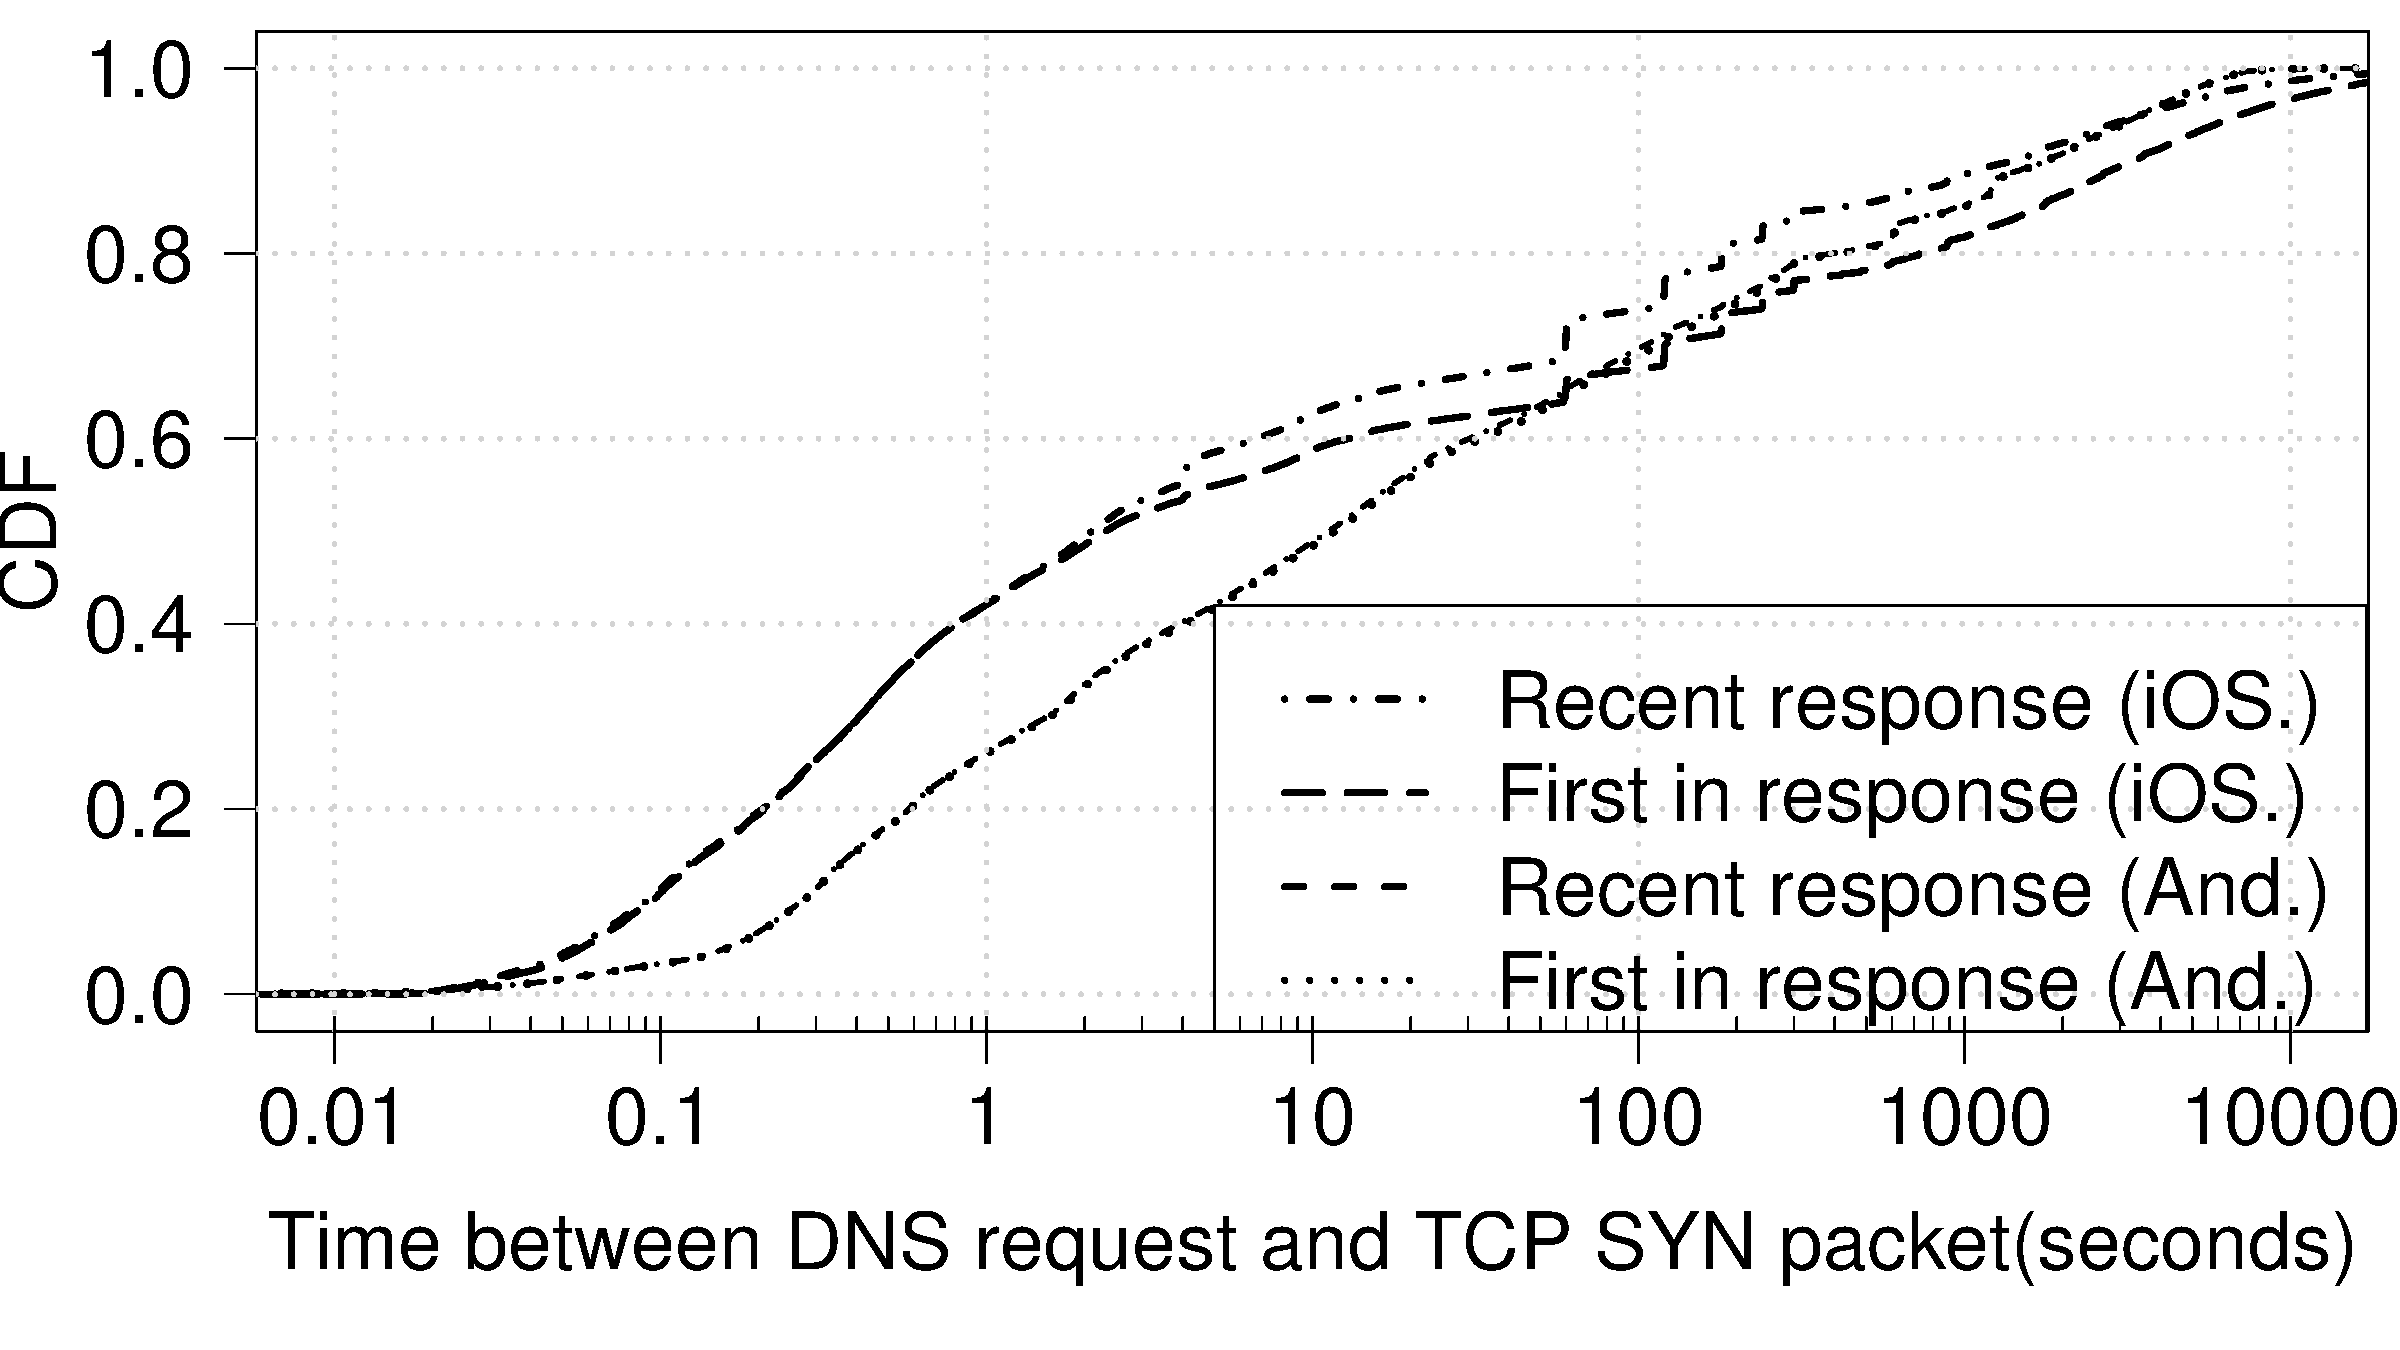
\includegraphics[width=\columnwidth]{plots/sslanalysis_dns_timediff_distrib.pdf}
% \caption{Distribution of the time between DNS response that contained the IP address of the SSL server and the SYN from the SSL flows. 
% \emph{The lack of difference in the curves for Android devices implies that the first entry in the most recent DNS response contained the IP address of the SSL flow.\tbd{rename xlab to DNS response.}}}
% \label{fig:ssl-dns-first-recent-distrib}
% \end{figure}

% To analyze the impact of the ambiguity, in \fref{fig:ssl-dns-first-recent-distrib} we plot the distribution of the time between the DNS response that contained the IP address and SYN packet from the SSL flow. 
% For this plot, we consider two types of DNS responses: the most recent DNS response that contain the IP address in the SSL flows, and the most recent DNS response that contained the IP address as the first entry in the DNS response. 
% We observe that for Android flows we do not observe a difference in the curves for the distribution, implying that the first entry in the most recent DNS response contained the IP address of the SSL flow.
% However, for iOS devices we observe a difference in the distribution when the time difference between the SYN and DNS response is larger than three seconds. 
% This difference creates an ambiguity which can be aggravated by caching of name resolution by the applications. 

We use the DNS flows that passed through \platname to further classify the SSL flows, a technique similar to DN-Hunter~\cite{bermudez:dnhunter}.
DN-Hunter relies on the most recent FQDN that corresponds to the IP address, however in our controlled experiments we observe Android and iOS devices prefer the the first entry in DNS response while resolving \emph{hostnames}.
Popular webservices such as google are known to use the same pool of IP addresses for various applications, for example the IP for gmail may also be used for search. 
In \fref{fig:ssl-classification-app-service} we present the fraction of SSL traffic where the most recent DNS response contained the IP address of the SSL flow in the first position. 
We observe that for the majority of SSL traffic by volume and flows can be classified by using the DNS responses. 

In summary, we use \platname to perform controlled experiments and in the wild measurements to characterize mobile Internet traffic. 
We use Bro to analyze the data and build on the output of bro to further classify HTTP flows and SSL flows to identify the source of the traffic. 
We now present the results of our experiments and measurements study. 


%%% Local Variables: 
%%% mode: latex
%%% TeX-master: "main"
%%% End: 


\section{Characterizing Mobile Traffic}
\label{sec:measurement-results}

%\subsection{Dataset Description}
%\label{sec:dataset-description}
%
%- IRB based study from September 2012. 
%- Full packet capture
%- Currently serves 20 devices from 14 users, 8 Android, 12 iOS device,    
%  4 iPads, 7 iPhones, and 1 iPod Touch.
%  15 service providers spread across US and France.
%- 30.2 GB of Traffic Volume from November 1, 2012

\subsection{Summary Statistics}
\label{sec:initial-results}

In this section, we use several descriptive statistics to 
summarize our dataset and provide context for the remainder 
of the section.

Objective  coverage of meddle across access technology and devices 

I plan to use these two tables to introduce the results in the
following sections.


\begin{table}
\begin{center}
\begin{tabular}{|l|l|r|r|r|r|}
\hline
\multirow{2}{*}{\bf Protocol} & \multirow{2}{*}{\bf Service} & \multicolumn{2}{|c|}{\bf Android} & \multicolumn{2}{|c|}{\bf iOS} \tabularnewline
\cline{3-6}
           &           &  \textbf{Flows}  &  \textbf{Bytes}  &  \textbf{Flows}  &  \textbf{Bytes}  \tabularnewline
\hline
 TCP       &  HTTP     &  14.87  &  74.31  &  16.07  &  82.01  \tabularnewline
\hline
TCP       &  SSL      &  37.19  &  24.35  &  37.64  &  17.31  \tabularnewline
\hline
 UDP       &  -        &  40.52  &   0.98  &  42.34  &   0.49  \tabularnewline
\hline
 TCP       &  other    &   2.08  &   0.22  &   1.13  &   1.89  \tabularnewline
\hline
 Other     &  -        &   5.35  &   0.14  &   2.82  &   0.09  \tabularnewline
\hline
\multicolumn{2}{|c|}{\emph{total}} & 100.00 & 100.00 & 100.00 & 100.00 \tabularnewline
\hline
\end{tabular}
\end{center}
\caption{Percentage of flows and bytes from iOS and Android devices. \tbd{Verify total 100
    for final results} \emph{SSL is responsible for the majority of
    TCP flows from iOS and Android devices.}} 
\label{tab:summaryIOSAndroidTraffic}
\end{table}

In \fref{tab:summaryIOSAndroidTraffic}.

We classify the IP flows as either TCP, UDP, or other; all IP flows
that cannot be classified as either TCP or UDP are classified as
other. We further classify TCP flows as either HTTP, SSL, or
other. The SSL flows include HTTPS, IMAP, and other services that rely
on SSL to secure the connection between the mobile client and the
remote server. TCP flows that are not classified
as either HTTP or SSL are classified as other.  

In our traces we observe that DNS is responsible for more 93.5\% of
the UDP flows. The rest of the flows are due to services such as
Skype which is not widely used by users in our dataset. 
%421310/449421 

HTTP is the dominant protocol of traffic. SSL flows outnumber the HTTP
flows however the bytes per SSL flow is significantly smaller than the
bytes per HTTP flow. This is because of the media content from
streaming sites such as YouTube and Netflix is streamed over HTTP. 

\begin{table}
\begin{center}
\begin{tabular}{|l|l|r|r|r|r|}
\hline
\multirow{2}{*}{\bf Protocol} & \multirow{2}{*}{\bf Service} & \multicolumn{2}{|c|}{\bf Wi-Fi} & \multicolumn{2}{|c|}{\bf Cellular} \tabularnewline
\cline{3-6}
           &           &  \textbf{Flows}  &  \textbf{Bytes}  &  \textbf{Flows}  &  \textbf{Bytes}  \tabularnewline
\hline
 TCP       &  HTTP     &  16.91  &  83.52  &  13.03  &  56.14  \tabularnewline
\hline
 TCP       &  SSL      &  38.18  &  15.83  &  36.14  &  41.42  \tabularnewline
\hline
UDP       &  -        &  41.43  &   0.49  &  41.56  &   1.67  \tabularnewline
\hline
TCP       &  other    &   1.38 &   0.16  &   1.95  &   0.4  \tabularnewline
\hline
Other     &  -        &   2.12  &  0.01  &   7.2  &   0.3  \tabularnewline
\hline
\multicolumn{2}{|c|}{\emph{total}} & 100.00 & 100.00 & 100.00 & 100.00 \tabularnewline
\hline
\end{tabular}
\end{center}
\caption{Percentage of flows and bytes using Wi-Fi and Cellular as access technology. \tbd{Verify total 100
    for final results} \emph{The share of SSL traffic over Cellular
    networks is larger than its share over Wi-Fi.}}  
\label{tab:summaryWifiCellularTraffic}
\end{table}


In \fref{tab:summaryWifiCellularTraffic}.

7.2 of cellular traffic classified as other is an artifact of our user base that includes
researchers who tend to troubleshoot connectivity issues using icmp packets.

Though the fraction of flows for HTTP over Wi-Fi and Cellular remain
the same, the byte shares are different. This is because Wi-Fi is the
prefered medium to transfer media content. The flows that transfer media content
typically have more bytes compared to flows that do not contain media
content. 

SSL traffic is typically compressed - discussion on compression
opportunities for HTTP over Cellular networks refer to section ... for
more details. We can refer to this section to introduce
compression.

The increase in HTTP traffic over Wi-Fi is also because apps such as
Google Plus (image backup on Android) allow users to upload their
images only over Wi-Fi.


\subsection{Case Study: Device Specific Apps (iOS Push)}
\label{sec:case-study-ios}

In this section we present the results of a detailed case study 
of iOS push. We focus on this application because it represents 
an OS-managed service on an operating system that received 
little research attention due to its closed-source nature. 

We set out to answer the following questions: (1) What is the 
empirical network impact of push notifications and does the 
measured activity coincide with published documentation?
(2) Using \meddle, is there any relevant data traffic that is 
not captured by the VPN tunnel? (3) What is the impact of 
a VPN connection on network behavior? (4) Can we use 
network traffic alone to infer the state of the device?

\noindent \textbf{iOS Push Under the Microscope.} 
The Apple Push Notification Service 
(APNS) implements push for iOS. The documentation for APNS provides limited details about 
the implementation, but does specify expected behavior (\eg push 
connections are established over cellular connections even if 
\wifi is available). 

We explicitly verified all provided documentation and confirmed that 
all statements are true with the exception of notification behavior 
with an iPad. The documentation states that the iPad will always 
remain associated with a \wifi AP, even if it is not plugged in. Our 
experience show this is not the case.

\tbd{Are we sure that devices are getting SMS notifications to connect to an apple server?}
When a push notification is received, the iOS device connects to port
5223 of a nearby Apple server. For each iOS device in our dataset we
logged the timestamp at which these connections were established. From
this set of connections we then selected the connections established
between midnight at 6 am of the users local time. For each user, we
computed the median of time interval between successive
connections. We observe this median to be in the range of 190 seconds
to 590 seconds. This time interval depends on the different apps for
which the user has enabled notifications. 
\tbd{Add figure}

A user can disable notifications for specific time intervals on
devices running iOS 6. In our dataset, three devices had notification
disabled during different time intervals. During these time intervals
we did not observe any traffic for notifications.

\noindent\textbf{Impact of a VPN and power state.}
In the remainder of this section we perform controlled experiments 
to understand the impact of a VPN connection, the power state and 
the available access technologies on the network traffic generated 
by APNS. In summary, we find that the impact of the VPN depends 
on the power state and access technology -- but there exist cases 
where the VPN does not noticeably change network traffic from APNS.
Further, we find that these changes in traffic patterns are relatively 
easy to identify, meaning we can use traffic from \meddle to infer 
when a device is plugged in and which access technologies are 
available.

All the following experiments are performed on an \iphone 4 with iOS
6.0.1.  At the beginning of each experiment we close all applications
and restart the \iphone{}. The \iphone{} is connected in \wifi{} to a
controlled access point on which we perform a tcpdump on the \wifi{}
interface and monitor the \wifi{} association between the access point
and the \iphone{}. Each experiment lasts for around 1 hour. 

\begin{figure}
\centering
        \includegraphics[width=0.8\linewidth]{../../code/pushNotification/Fig/bw_iphone_wifi_3g_plug_novpn_interTs.eps}
  \caption{Distribution of the interarrival times of Ethernet frames
    for a one hour experiment with an idle \iphone{} plugged-in, with \wifi{} and 3G
    enabled, and no VPN enabled. For each bin of 1 second, we count
    the number of interarrivals in that bin.}
  \label{fig:push_w3p_interTs}
\end{figure}

%\begin{figure}
%\centering
%        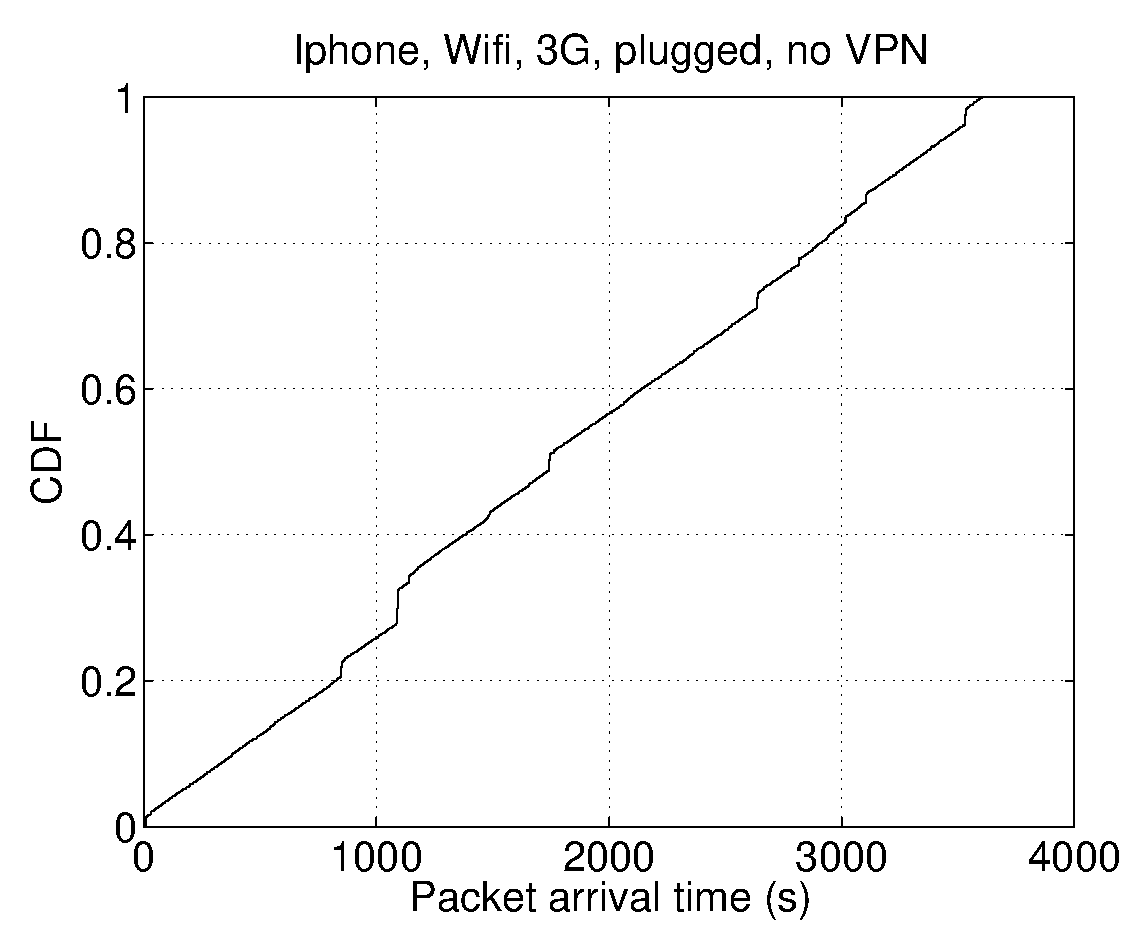
\includegraphics[width=0.8\linewidth]{../../code/pushNotification/Fig/bw_iphone_wifi_3g_plug_novpn_ts.eps}
%        \caption{Cumulative distribution of the Ethernet frames
%          arrival with time for a one hour experiment with an idle
%          \iphone{} plugged-in, with \wifi{} and 3G enabled, and no VPN
%          enabled.}
%  \label{fig:push_w3p_ts}
%\end{figure}

\begin{figure}
\centering
        \includegraphics[width=0.8\linewidth]{../../code/pushNotification/Fig/bw_iphone_wifi_3g_plug_vpn_interTs.eps}
  \caption{Distribution of the interarrival times of Ethernet frames
    for a one hour experiment with an idle \iphone{} plugged-in, with \wifi{} and 3G
    enabled, and VPN enabled. For each bin of 1 second, we count
    the number of interarrivals in that bin.}
  \label{fig:push_w3pv_interTs}
\end{figure}

%\begin{figure}
%\centering
%        \includegraphics[width=0.8\linewidth]{../../code/pushNotification/Fig/bw_iphone_wifi_3g_plug_vpn_ts.eps}
%  \caption{Cumulative distribution of the Ethernet frames
%          arrival with time for a one hour experiment with an idle
%          \iphone{} plugged-in, with \wifi{} and 3G enabled, and VPN
%          enabled.}
%  \label{fig:push_w3pv_ts}
%\end{figure}

\emph{Behavior when plugged in.} When an \iphone{} is plugged-in, it always remains associated with the
\wifi{} access point if \wifi{} is enabled on the device. We performed
a first set of experiments to observe the traffic to and from an idle
\iphone{}. We see in Fig.~\ref{fig:push_w3p_interTs} and
Fig.~\ref{fig:push_w3pv_interTs} that the largest interarrival between
two frames is in the order of 10 seconds for both the VPN and no VPN
scenarios. We also observe no noticeable difference in the arrival of
frames with time for both the VPN (see Fig.~\ref{fig:push_w3pv_ts} and
no VPN (see Fig.~\ref{fig:push_w3p_ts}) scenarios. \emph{Thus, it 
appears that the VPN connection has no noticeable impact on 
network traffic generated for APNS when the device is plugged in.}

%We don't claim this
%traffic to be typical, in particular, our access point is a Windows 7
%machine sending SSDP traffic to announce available services. Instead,
%we use it to understand in our experimental setup the background
%traffic.

%\begin{figure}
%\centering
%        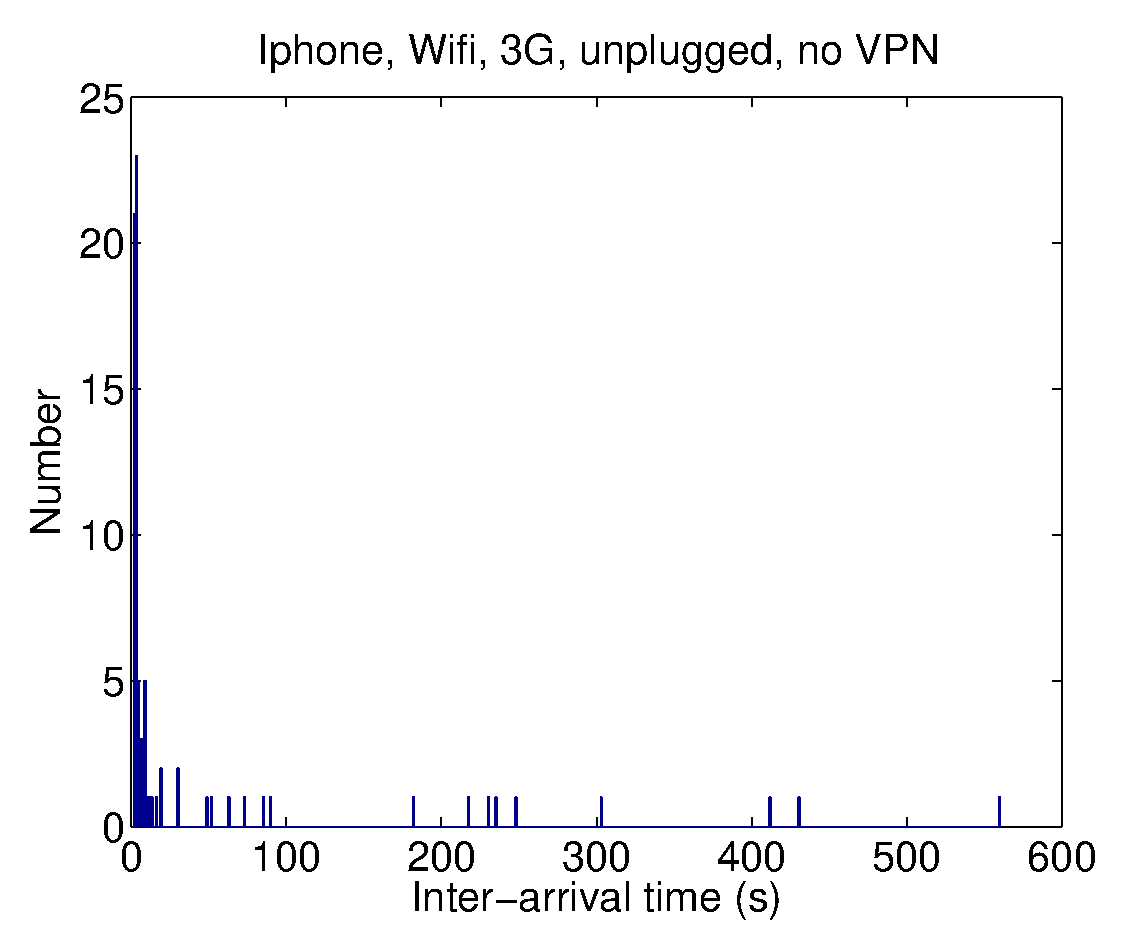
\includegraphics[width=0.8\linewidth]{../../code/pushNotification/Fig/bw_iphone_wifi_3g_unplug_novpn_interTs.eps}
%  \caption{Distribution of the interarrival times of Ethernet frames
%    for a one hour experiment with an idle \iphone{} unplugged, with \wifi{} and 3G
%    enabled, and no VPN enabled. For each bin of 1 second, we count
%    the number of interarrivals in that bin.}
%  \label{fig:push_w3_interTs}
%\end{figure}

\begin{figure}
\centering
        \includegraphics[width=0.8\linewidth]{../../code/pushNotification/Fig/bw_iphone_wifi_3g_unplug_novpn_ts.eps}
  \caption{Cumulative distribution of the Ethernet frames
          arrival with time for a one hour experiment with an idle
          \iphone{} unplugged, with \wifi{} and 3G enabled, and no VPN
          enabled.}
  \label{fig:push_w3_ts}
\end{figure}

\emph{Behavior when on battery.} 
In a second set of experiments, we consider a default \iphone{}
setting with 3G and \wifi{} enabled, and the \iphone{} unplugged. This
corresponds to a typical setting for a user on move.  We observe in
Fig.~\ref{fig:push_w3_interTs} some very large interarrival
times for frames. All interarrival times larger than 10 seconds correspond to
periods during which the \wifi interface of the \iphone{} is not
associated to the access point for energy saving. 




%\begin{figure}
%\centering
%        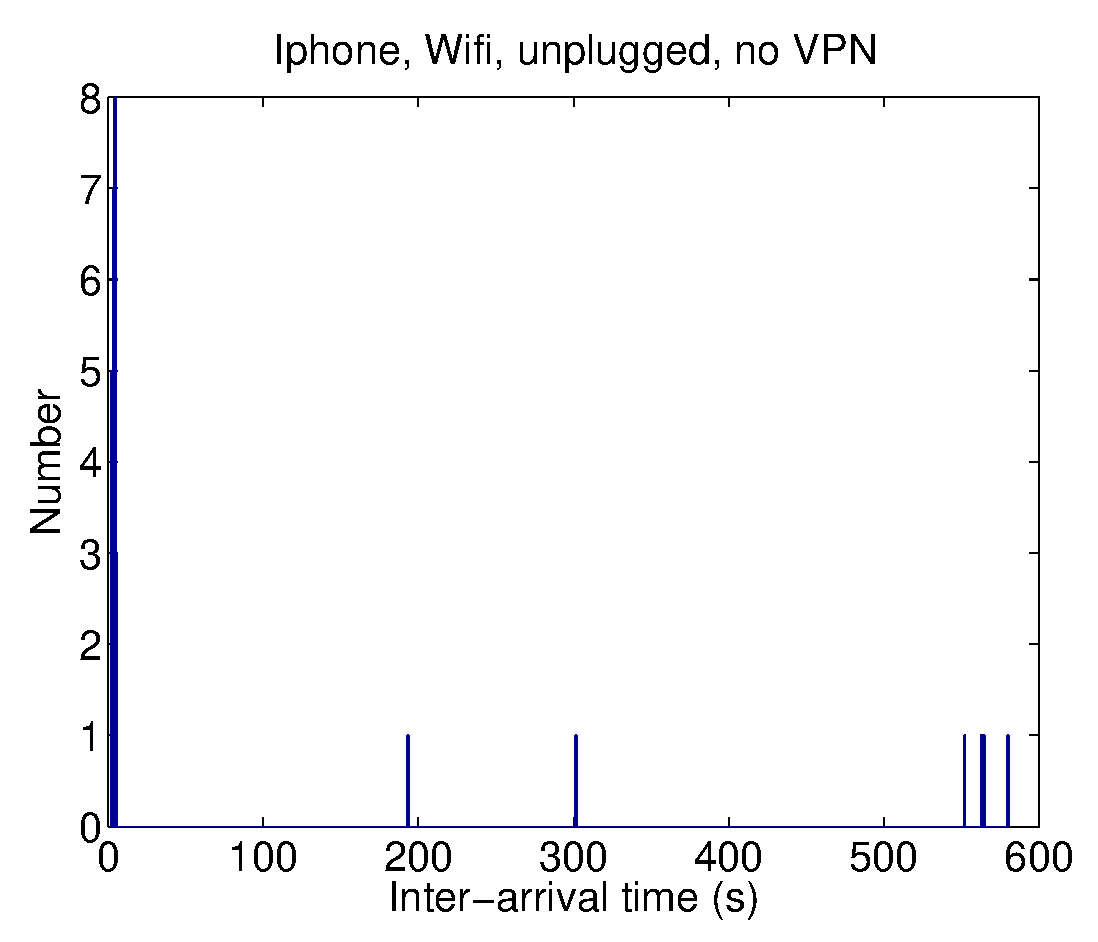
\includegraphics[width=0.8\linewidth]{../../code/pushNotification/Fig/bw_iphone_wifi_unplug_novpn_interTs.eps}
%  \caption{Distribution of the interarrival times of Ethernet frames
%    for a one hour experiment with an idle \iphone{} unplugged, with \wifi{} 
%    enabled, and no VPN enabled. For each bin of 1 second, we count
%    the number of interarrivals in that bin.}
%  \label{fig:push_w_interTs}
%\end{figure}

\begin{figure}
\centering
        \includegraphics[width=0.8\linewidth]{../../code/pushNotification/Fig/bw_iphone_wifi_unplug_novpn_ts.eps}
  \caption{Cumulative distribution of the Ethernet frames
          arrival with time for a one hour experiment with an idle
          \iphone{} unplugged, with \wifi{} enabled, and no VPN
          enabled.}
  \label{fig:push_w_ts}
\end{figure}

Surprisingly, even though \iphone{} is idle, the traffic pattern
is not regular (Fig.~\ref{fig:push_w3_ts}). To
understand this irregularity, we made a new experiment with 3G
disabled. We observe in Fig.~\ref{fig:push_w_interTs} that the largest
interarrival is still in the order of 550 seconds, as in the case with
3G enabled, but we have less variety in the interarrival times. This
is confirmed by Fig.~\ref{fig:push_w_ts} that shows a regular
succession of short periods during which frames are received and long
periods during which the wifi connection is not associated to the
access point.

Therefore, there is an evidence that the 3G connection might trigger
the association of the \iphone{} \wifi interface with the access
point. This is confirmed by experiments we performed with iMessage
that is using the push notification infrastructure of Apple. When both
3G and \wifi{} are enabled on an \iphone{}, a permanent connection to
the push notification infrastructure of Apple is setup on the 3G
interface. Each time an iMessage is received, it is piggybacked on the
push notification message (when short enough). Interestingly, the \wifi{}
interface is always woken-up even if no payload is sent on it. \tbd{Is it 
fair to say this is wasted energy?}

In conclusion, there is evidence that some APNS signaling occurs 
outside of the packet-switched network. Thus, though \meddle appears 
to capture all IP traffic it may miss traffic in the circuit switched network 
that, in turn, causes IP traffic to occur.

%We observed this same behavior on the tcpdump traces used to plot
%Fig.~\ref{fig:push_w3_ts}. We observe that the \wifi{} interface is
%woken-up (we observe a specific ARP and DHCP exchange that takes place
%for each \wifi{} association to the access point), but no payload is
%exchanged. In this case, as we do not use a VPN, we cannot monitor the
%3G traffic using \meddle{}, but we guess that traffic received on the
%3G interface trigger the wake of the \wifi{} interface. We plan to
%further explore this issue. 

%\begin{figure}
%\centering
%        \includegraphics[width=0.8\linewidth]{../../code/pushNotification/Fig/bw_iphone_wifi_unplug_vpn_interTs.eps}
%  \caption{Distribution of the interarrival times of Ethernet frames
%    for a one hour experiment with an idle \iphone{} unplugged, with \wifi{}
%    enabled, and VPN enabled. For each bin of 1 second, we count
%    the number of interarrivals in that bin.}
%  \label{fig:push_wv_interTs}
%\end{figure}




\emph{Behavior when switching access technologies.} We performed a third set of experiments with the VPN enabled. This set
of experiment shows the impact of using \meddle on the traffic pattern
and the power management policy. We see in
Fig.~\ref{fig:push_wv_interTs} and Fig.~\ref{fig:push_wv_ts} that
there is no noticeable differences when enabling \meddle with \wifi{} only. However,
when enabling both \wifi and 3G the frames interarrival time
(Fig.~\ref{fig:push_w3v_interTs}) and the cumulative arrival of frames
(Fig.~\ref{fig:push_w3v_ts}) is significantly different. 
\tbd{It will probably be too short for the deadline, but I need to see
on the meddle logs what are these 3G messages. I cannot get them from
my setup. I guess that the VPN is using keep alive message every 45
seconds. As the 3G connection never sleep, receiving such a packet
trigger the wake-up of the \wifi{} interface. When 3G is disabled, the
keep alive messages cannot prevent the \wifi{} interface to
sleep. Ashwin, if you are aware of such a timer in your VPN config, we
can safely state my guess in the paper.}

\begin{figure}
\centering
        \includegraphics[width=0.8\linewidth]{../../code/pushNotification/Fig/bw_iphone_wifi_unplug_vpn_ts.eps}
  \caption{Cumulative distribution of the Ethernet frames
          arrival with time for a one hour experiment with an idle
          \iphone{} unplugged, with \wifi{} enabled, and VPN
          enabled.}
  \label{fig:push_wv_ts}
\end{figure}

\begin{figure}
\centering
        \includegraphics[width=0.8\linewidth]{../../code/pushNotification/Fig/bw_iphone_wifi_3g_unplug_vpn_ts.eps}
  \caption{Cumulative distribution of the Ethernet frames
          arrival with time for a one hour experiment with an idle
          \iphone{} unplugged, with \wifi{} and 3G enabled, and VPN
          enabled.}
  \label{fig:push_w3v_ts}
\end{figure}

\subsection{Case Study Longitudinal Measurements - Google Search }
\label{sec:case-study-google}



% 1353489965.972204       7S1qUBBGGUg     24.19.59.238    45867   173.194.79.138  80      1       GET     suggestqueries.google.com       /complete/search?hl=en&ds=yt&client=androidyt&hjson=t&oe=UTF-8&q=a      -       Apache-HttpClient/UNAVAILABLE (java 1.4)        0       356     200     OK      -       -       -       (empty) -       -       -       -       -       application/json; charset=UTF-8 chunked text/plain      -       -
% 1353489966.199133       7S1qUBBGGUg     24.19.59.238    45867   173.194.79.138  80      2       GET     suggestqueries.google.com       /complete/search?hl=en&ds=yt&client=androidyt&hjson=t&oe=UTF-8&q=aw     -       Apache-HttpClient/UNAVAILABLE (java 1.4)        0       321     200     OK      -       -       -       (empty) -       -       -       -       -       application/json; charset=UTF-8 chunked text/plain      -       -
% 1353489966.471227       7S1qUBBGGUg     24.19.59.238    45867   173.194.79.138  80      3       GET     suggestqueries.google.com       /complete/search?hl=en&ds=yt&client=androidyt&hjson=t&oe=UTF-8&q=awe    -       Apache-HttpClient/UNAVAILABLE (java 1.4)        0       300     200     OK      -       -       -       (empty) -       -       -       -       -       application/json; charset=UTF-8 chunked text/plain      -       -
% 1353489966.881255       7S1qUBBGGUg     24.19.59.238    45867   173.194.79.138  80      4       GET     suggestqueries.google.com       /complete/search?hl=en&ds=yt&client=androidyt&hjson=t&oe=UTF-8&q=awes   -       Apache-HttpClient/UNAVAILABLE (java 1.4)        0       301     200     OK      -       -       -       (empty) -       -       -       -       -       application/json; charset=UTF-8 chunked text/plain      -       -
% 1353489967.365324       7S1qUBBGGUg     24.19.59.238    45867   173.194.79.138  80      5       GET     suggestqueries.google.com       /complete/search?hl=en&ds=yt&client=androidyt&hjson=t&oe=UTF-8&q=aweso  -       Apache-HttpClient/UNAVAILABLE (java 1.4)        0       302     200     OK      -       -       -       (empty) -       -       -       -       -       application/json; charset=UTF-8 chunked text/plain      -       -
% 1353489968.001541       7S1qUBBGGUg     24.19.59.238    45867   173.194.79.138  80      6       GET     suggestqueries.google.com       /complete/search?hl=en&ds=yt&client=androidyt&hjson=t&oe=UTF-8&q=awesom -       Apache-HttpClient/UNAVAILABLE (java 1.4)        0       303     200     OK      -       -       -       (empty) -       -       -       -       -       application/json; charset=UTF-8 chunked text/plain      -       -
% 1353489968.303481       7S1qUBBGGUg     24.19.59.238    45867   173.194.79.138  80      7       GET     suggestqueries.google.com       /complete/search?hl=en&ds=yt&client=androidyt&hjson=t&oe=UTF-8&q=awesome        -       Apache-HttpClient/UNAVAILABLE (java 1.4)        0       304     200     OK      -       -       -       (empty) -       -       -       -       -       application/json; charset=UTF-8 chunked text/plain      -       -
% 1353489968.469449       7S1qUBBGGUg     24.19.59.238    45867   173.194.79.138  80      8       GET     suggestqueries.google.com       /complete/search?hl=en&ds=yt&client=androidyt&hjson=t&oe=UTF-8&q=awesome+       -       Apache-HttpClient/UNAVAILABLE (java 1.4)        0       330     200     OK      -       -       -       (empty) -       -       -       -       -       application/json; charset=UTF-8 chunked text/plain      -       -
% 1353489969.221635       7S1qUBBGGUg     24.19.59.238    45867   173.194.79.138  80      9       GET     suggestqueries.google.com       /complete/search?hl=en&ds=yt&client=androidyt&hjson=t&oe=UTF-8&q=awesome+t      -       Apache-HttpClient/UNAVAILABLE (java 1.4)        0       345     200     OK      -       -       -       (empty) -       -       -       -       -       application/json; charset=UTF-8 chunked text/plain      -       -
% 1353489969.551634       7S1qUBBGGUg     24.19.59.238    45867   173.194.79.138  80      10      GET     suggestqueries.google.com       /complete/search?hl=en&ds=yt&client=androidyt&hjson=t&oe=UTF-8&q=awesome+to     -       Apache-HttpClient/UNAVAILABLE (java 1.4)        0       390     200     OK      -       -       -       (empty) -       -       -       -       -       application/json; charset=UTF-8 chunked text/plain      -       -
% 1353489969.953698       7S1qUBBGGUg     24.19.59.238    45867   173.194.79.138  80      11      GET     suggestqueries.google.com       /complete/search?hl=en&ds=yt&client=androidyt&hjson=t&oe=UTF-8&q=awesome+to+    -       Apache-HttpClient/UNAVAILABLE (java 1.4)        0       383     200     OK      -       -       -       (empty) -       -       -       -       -       application/json; charset=UTF-8 chunked text/plain      -       -


\begin{table}
\begin{center}
\begin{tabular}{|c|c|l|}
\hline
Time & Bytes & Query \tabularnewline
 & Downloaded & String\tabularnewline
\hline 
1353489965.97 & 356 & a \tabularnewline
\hline
1353489966.19& 321 & aw\tabularnewline
\hline
1353489966.47& 300 & awe\tabularnewline
\hline
1353489966.88& 301 & awes\tabularnewline
\hline
1353489967.36& 302 & aweso\tabularnewline
\hline
\end{tabular}
\end{center}
\caption{Table}
\label{tab:ExampleGoogleSearch}
\end{table}
We now use Google search as an example of longitudinal studies that
are possible using using Meddle.

In \fref{tab:ExampleGoogleSearch} we present a sample search session on
Android 4.0. During this sesssion, we observe that each key stroke by
the user resulted in a unique GET query made to a Google server. We
observe similar behavior on Android 4.0, Android 4.1, and Android 4.2
\tbd{confirm}. In the case of iOS devices we observed search queries
in the clear on devices running iOS 5. On devices running iOS 6 we
observe that search queries take place over SSL. \tbd{Privacy similar
  to desktop sentence.}


\subsection{Case Study Filtering Intrusive Traffic}
\label{sec:case-study-filtering}

\subsection{Case Study Traffic Optimization - Compression}
\label{sec:case-study-compression}

\subsection{Case Study Suspicious Apps}
\label{sec:case-study-susp}









 




%%% Local Variables: 
%%% mode: latex
%%% TeX-master: "main"
%%% End: 


\section{Related Work}
\label{sec:related}

Placeholder for the papers.
\cite{thiagarajan:mobbat}

\cite{balasubramanian:encon}

\cite{vallina-rod:ads}

\cite{falaki:mobileusage}

Bro port based classification of HTTP, SSL, other, and so on. 


\section{Classification of Application}

\platname enables us to monitor the data being exchanged by the mobile device. 
However, it does not provide any details of the source of the data. 
We use the following technique to estimate the source of the mobile data traffic. 
In \ref{tab:summaryIOSAndroidTraffic} and \ref{tab:summaryWifiCellularTraffic} we observe that TCP is responsible for the majority of the traffic volume from iOS and Android devices regardless of the access technology used. 
We therefore focus on associating TCP flows to the applications for our analysis. 
From our analysis we were able to classify \tbdv{x\%} of the TCP traffic volume and \tbdv{y\%} of the TCP flows to the applications.

\subsection{Methodology}

\subsection{Results}

User Agent based classification
flows per user with a blank user agent. 
flows per user with a default user agent 
flows with application in user agent


SSL certificate based classification
flows to dedicated hosts
flows to cdns

\subsection{Discussion}

\section{Specific application behavior}


\section{Ads and Analytics}

Ads and Analytic sites have received considerable attention.
The reason for the attention being the intrusiveness exhibited by the ads and analytics sites in tracking personal information. 
\cite{vallina-rod:ads} show that \tbdv{ } of data traffic volume observed from a Cellular ISP is because of mobile ads. 
In our traces we use the classification of \cite{vallina-rod:ads} and \cite{YoyoAds} to classify flows as ads flows. 



\section{Discussion on Platform}

IPv6 support of VPNs

ISP support of VPNs. One ISP blocked VPN access. 

Open source ??

Releasing datasets ??


